\documentclass[../delivery_hospital_report.tex]{subfiles}
\graphicspath{ {images/}{../images/}{../../images/} }

\begin{document}
\chapter{Integração Software Hardware}

Todos os algoritmos complexos desenvolvidos para robô hospitalar são feitos com linguagem de alto nível, com Python \cite{python21}, ou C++ \cite{c++21} em algumas situações. Porém, como esses algoritmos requerem um poder computacional muito maior que um microcontrolador embarcado consegue fornecer, é necessário utilizar um computador embarcado para realizar essas diversas operações complexas e processar os dados.

\begin{figure}[h]
\centering
    \caption{Integração da Jetson com Módulos Embarcados}
    \centering % para centralizarmos a figura
    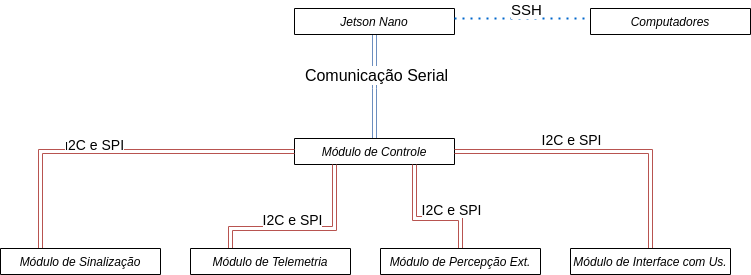
\includegraphics[width=14cm]{integracao.png}
    \caption*{Fonte: Elaborada pelo autor}
    \label{figura:}
\end{figure}

Por outro lado, a integração de todo o Software do sistema tem uma série de desafios, porém os mais importantes no ponto que projeto esta é: A utilização , Conexão a distância  e se comunicar com os microcontroladores com o Computador embarcado.

\section{Computador Embarcado}
A escolha do computador embarcado é fundamental  para o projeto, pois o mesmo é o grande limitador do poder computacional do robô completo. A escolha errado desse computador corrobora para o mal funcionamento de todo o hardware e software, dado que conforme a complexidade aumentasse, a velocidade de processamento de dados cairia até um ponto que o robô entraria em colapso computacionalmente.

De maneira geral, ainda como herança da primeira versão do robô hospitalar, o computador embarcado utilizado no projeto foi a Jetson Nano Develop Kit \cite{jetson21}. O motivo completo da escolha desse computador embarcado, a qual eu não presenciei, pode ser visto no relatório do João Pedro Secchim Sotto Maior \cite{sotto_rel20}. O motivo da escolha pode ser visto abaixo:

\begin{citacaoLonga}
	Nos últimos anos houve grandes avanços no desenvolvimento de processadores arm, principalmente por ser a arquitetura utilizada nos smartphones e tablets. Aproveitando esses avanços diversas empresas desenvolveram computadores que utilizam esses processadores, a mais conhecida é a fundação Raspberry Pi que produz e vende o Raspberry Pi, single-board computer (computador de placa única) que é um computador que possui todos os componentes que precisa soldados em uma única placa. 
	
	Após pesquisar as opções de computadores disponíveis, foi necessário escolher entre três placas, o Raspberry Pi, o Labrador desenvolvido na Escola Politécnica da USP [4] ou uma placa da linha Jetson da Nvidia [5]. Uma das razões que motivou a decisão de utilizar uma placa da linha Jetson da Nvidia foi grande presença da empresa na área de Machine learning e Computer vision. Além disso, os computadores da linha Jetson possuem GPUs muito mais poderosas do que as outras duas opções apresentadas, o que acelera muito o processo de manipulação de imagens.
\end{citacaoLonga}

No mais, desde a escolha da Jetson Nano, não houve nenhuma necessidade até o momento de trocar o computador embarcado, muito pelo contrário, ele ainda está suprindo muito bem as demandas computacionais do projeto.

\begin{figure}[h]
\centering
    \caption{Jetson Nano Develorper Kit}
    \centering % para centralizarmos a figura
    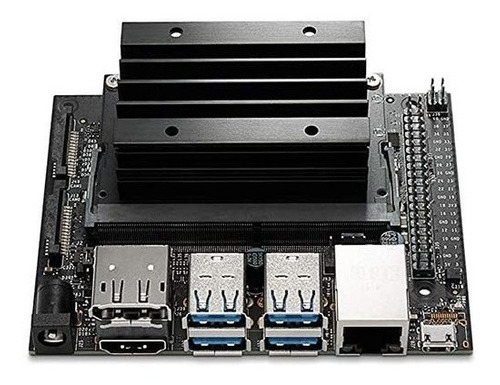
\includegraphics[width=10cm]{jetson_nano.jpg}
    \caption*{Fonte: Nvidia}
    \label{figura:1° Versão Robô Hospitalar}
\end{figure}


\section{Conexão a distância}

A Jetson Nano \cite{jetson21} é um computador embarcado que no projeto do robô hospitalar tem a missão de carregar os códigos de controle de todo o robô autônomo. No mais, quando surge necessidade mexer nessa parte do hardware do robô, não é muito interessante precisar desmontar uma série de equipamentos para ter acesso a Jetson. Tendo isso em mente, surge a necessidade de conseguir acessar o computador embarcado a distância.

Para resolver esse problema na Jetson Nano, foi implementado a comunicação Secure Shell (SSH) \cite{ssh21},  que é um protocolo de rede criptográfico para operação de serviços de rede de forma segura sobre uma rede insegura. Além de ser extremamente seguro, o protocolo SSH não demanda de uma boa conexão de internet para ter uma respostas satisfatória, um dos requisitos mais importantes, levando em consideração que dentro do hospital universitário a conexão com a rede wireless não é boa no estabelecimento todo.

\begin{figure}[h]
\centering
    \caption{Comunicação SSH}
    \centering % para centralizarmos a figura
    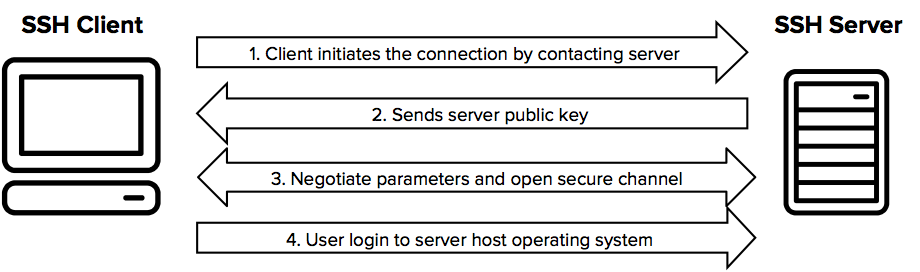
\includegraphics[width=14cm]{ssh_conection.png}
    \caption*{Fonte: Imagem obtida em hostinger.com.br}
    \label{figura:}
\end{figure}

A implementação é relativamente simples, basta ter o ssh devidamente instalado na Jetson Nano e no computador que deseja acessar remotamente. No caso da Jetson, como se comporta como servidor, é necessário criar uma chave SSH, de resto, a implementação é idêntica em ambos os dispositivos. 

\section{Comunicação com Embarcados}

A comunicação seria capaz de enviar e receber toda a informação sequencialmente, o que abre a possibilidade que o número de fios seja menor. Em outras palavras, protocolos de comunicação baseados no serial, são síncronos, ou seja, dependem do clock do sistema. Por outro lado, diferente de protocolos de comunicação, só consegue se comunicar com um aparelho por vez.

Outros protocolos de comunicação, como I2C e SPI, o qual as conexões são organizadas de forma paralelo, ou seja , é capaz de enviar e receber dados em mais de uma via de comunicação, assim, é capaz de enviar vários bits simultaneamente, resultando em maior rapidez na transmissão da informação.

\begin{figure}[h]
\centering
    \caption{Comunicação Serial}
    \centering % para centralizarmos a figura
    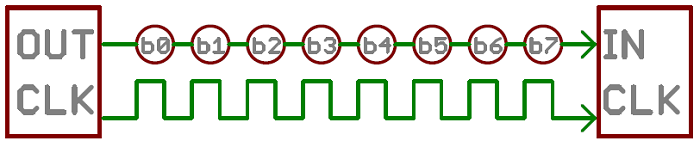
\includegraphics[width=14cm]{serial_communication.png}
    \caption*{Fonte: Obtido em https://www.robocore.net/}
    \label{figura:Comunicação Serial}
\end{figure}

No nosso caso, como só precisamos nos comunicar com um microcontrolador e como protocolo serial é mais simples de se implementar do que os outros protocolos, por decisão de projeto foi adotado a comunicação serial para haver essa ponte entre os dados processados na jetson para os módulos embarcados.

\end{document}

